
\documentclass{article}
    \usepackage[utf8]{inputenc}
    \usepackage{comment}
    \usepackage{environ}
    \usepackage{listings}
    \usepackage{xcolor}
    \usepackage[letterpaper, portrait, margin=1in]{geometry}
    \usepackage{amsmath}
    \usepackage{amssymb}
    \usepackage{graphicx}
    \usepackage{hyperref}
    
    \newif\ifshowsolutions
    
    % comment the following line to hide solutions
    \showsolutionstrue
    
    \ifshowsolutions
        \newenvironment{solution}{

            \color{blue} \smallskip \textbf{Solution:}}{}
    \else
        \NewEnviron{solution} {
            \ \\
            \ \\
            \ \\
        }
    \fi
    
    \begin{document}
    
    \part*{Continuous Probability, Joint Distributions}
    \vspace{-7pt}
    \hrule
    \vspace{7pt}
    \section{Intro}
    \begin{enumerate}
        \item How do continuous variables differ from discrete variables?
        \begin{solution}
            Both take values in $\mathbb{R}$. However, continuous variables have `enough outcomes' in the probability space to be uncountable.

            Discrete variables are defined in terms of a probability function $P(X = k)$
        \end{solution}
        \item How do we take expectation and variance for continuous variables?
        \begin{solution}
            \[
                E[X] = \int_{-\infty}^{\infty} x f_X(x) dx 
            \]
            \[
                E[X^2] = \int_{-\infty}^{\infty} x^2 f_X(x) dx
            \]
            In general for any function of a random variable $\varphi(x)$:
            \[  
                E[\varphi(X)] = \int_{-\infty}^{\infty} \varphi(x) f_X(x) dx
            \]
        \end{solution}
        \item What are the analogs of the following distributions for continuous random variables?
        \begin{enumerate}
            \item Uniform distribution
            \begin{solution}
                Still the uniform distribution, but just defined on a continuous probability space.
            \end{solution}
            \item Geometric distribution
            \begin{solution}
                The exponential distribution. It has the memoryless property like the geometric distribution.
            \end{solution}
            \item Binomial distribution
            \begin{solution}
                The normal/Gaussian distribution -- sort of. It has an easy-to-find mean and variance, and maintains a nice bell curve shape. But it can be negative as well.
            \end{solution}
        \end{enumerate}
        \item What are the properties of the CDF? Of the PDF? How do we get one from the other?
        \begin{solution}
            CDF: $P(X \leq x) = F(x) = \int_{-\infty}^x f_X(x) dx$

            PDF: $f_X(x) = F'(x)$.

            The CDF must be between 0 and 1, the limit to the left must be 0, and the limit to the right must be 1.
            The PDF must be $\geq 0$, and $\int_{-\infty}^{\infty} f_X(x) dx = 1$.
        \end{solution}
        \item Show how we can write every normal distribution in terms of the standard normal $N(\mu=0, \sigma^2=1)$.
        \begin{solution}
            Let the distribution be $X \sim N(\mu, \sigma^2)$. Then $E[X] = \mu$ and $var[X] = \sigma^2$. Consider \[
                \sigma N(0, 1) + \mu
            \].
            Then this has the same expectation and variance as $X$ and is normally distributed, so then $X = \sigma N(0, 1) + \mu$, and we get \[
                N(0, 1) = \frac{X - \mu}{\sigma}
            \]
        \end{solution}
    \end{enumerate}
        \section{Problems}
    \begin{enumerate}
        \item Let X be a random variable with pdf given by \[
            f_X(x) = \begin{cases}
                cx^2 & \text{if } |x| < 1 \\
                0 & \text{otherwise}
            \end{cases}
        \].
        \begin{enumerate}
            \item Find $c$ that makes this a valid random variable.
            \begin{solution}
            We want $\int_{-\infty}^\infty f_X(x) dx = 1$. So $\int_{-1}^1 cx^2 = c \left[\frac{1}{3} x^3\right]^{1}_{-1} = \frac{2}{3}c = 1$. Then $c = \frac{3}{2}$.
            \end{solution}
            \item Find $E[X]$ and $var[X]$.
            \begin{solution}
            \[
                E[X] = \int_{-1}^{1} x \cdot \frac{3}{2} x^2 dx = \frac{3}{2} \left[\frac{1}{4} x^4\right]^{1}_{-1} = 0
            \]
            This turns out to be $0$! This is because $(-x)^3 = - x^3$, also known as saying $x^3$ is an \textit{odd} function.

            To find $var[X] = E[X^2] - E[X]^2$, we first find $E[X^2]$: \[
                E[X^2] = \int_{-1}^{1} x^2 \cdot \frac{3}{2} x^2 dx = \frac{3}{2} \left[\frac{1}{5} x^5\right]^{1}_{-1} = \frac{3}{5}
            \]
            So our variance is just $\frac{3}{5}$.
            \end{solution}
            \item Find $P(X \leq \frac{1}{2})$.
            \begin{solution}
            We need to find $\int_{-\infty}^{\frac{1}{2}} f_X(x) dx$: \[
                P(X \leq \frac{1}{2}) = \int_{-1}^{\frac{1}{2}} \frac{3}{2}x^2 dx = \frac{3}{2} \left[\frac{1}{3}x^3\right]^{\frac{1}{2}}_{-1} = \frac{9}{16}
            \]
            \end{solution}
        \end{enumerate}
        \item Let $X$ be a random variable with pdf \[
            f_X(x) = \begin{cases}
                4x^3 & \text{if } 0 \leq x \leq 1 \\
                0 & \text{otherwise}
            \end{cases}
        \]
        Find $P(X \leq \frac{2}{3} \mid X > \frac{1}{3})$.
        \begin{solution}
            This is finding a conditional probability. We know: \[
                P(X \leq \frac{2}{3} \mid X > \frac{1}{3}) = \frac{P(X \leq \frac{2}{3} \cap X > \frac{1}{3})}{P(X > \frac{1}{3})} = \frac{P(\frac{1}{3} < X < \frac{2}{3})}{P(X > \frac{1}{3})}
            \]
            The rest is evaluating integrals, the top is $\int_{\frac{1}{3}}^{\frac{2}{3}}$ and the bottom is $\int_{\frac{1}{3}}^1$.
        \end{solution}
        \item Two real numbers are chosen uniformly from $[0,1]$. What is the probability that their sum is less than or equal to 1 given that one of them is less than or equal to 1/2?
        \begin{solution}
            It's really best to see the solution in a picture. We want to find: \[
                P(X + Y \leq 1 \mid X \leq \frac{1}{2} \cup Y \leq \frac{1}{2})
            \]
            We can summarize this with a diagram like this one:

            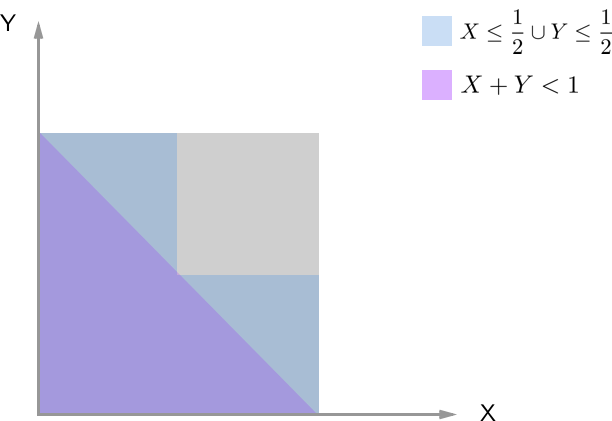
\includegraphics[height=5cm]{conditional-figure}

            Then this comes down to comparing areas. The area of where $X + Y < 1$ is $\frac{1}{2}$, while for $X \leq \frac{1}{2} \cup Y \leq \frac{1}{2}$
        \end{solution}
        \item Let $X$ and $Y$ be jointly continuous r.vs. with joint PDF \[
            f_{X,Y}(x, y) = \begin{cases}
                6e^{-(2x+3y)} & \text{if } x, y \geq 0 \\
                0 & \text{otherwise}
            \end{cases}
        \].
        Are $X$ and $Y$ independent? Find $P(X > Y)$.
        \begin{solution}
            Yes, they are. We can write \[
                f_{X,Y}(x, y) = 6e^{-(2x+3y)} = 6e^{-2x} 6e^{-2y} = f_X(x) f_Y(y)
            \]
            because we were able to factor the joint distribution into a product of the distributions of $X$ and $Y$, this means they are independent.

            Then finding $P(X > Y)$ becomes finding the integral of $f_{X, Y}(x, y)$ over all points where $X > Y$. This is basically splitting the first quadrant of the plane (where $x, y \geq 0$) into two halves along the diagonal, and we are interested in
            finding the integral over the bottom one. \[
                \int_{0}^\infty \int_{0}^x 6e^{-2x + 3y} dy dx 
            \]
            CS 70 doesn't expect you to evaluate integrals like this one. Sorry if I scared anybody. Almost every time, questions on continuous joint distributions are just about finding the area of
            shapes we know the formulas for, like problem 3.
        \end{solution}
        \item Let $X$ be a positive continuous r.v. Show that $E[X] = \int_{0}^\infty P(X \geq x) dx$.
        \begin{solution}
        I realized that this problem does not really help us that much. If you are interested, you can read more here: \url{https://math.stackexchange.com/questions/63756/tail-sum-for-expectation}
        \end{solution}
    \end{enumerate}
    \end{document}
        